%%%%% --------------------------------------------------------------------------------
%%
%%                               Document Template
%%
%%%%% --------------------------------------------------------------------------------
%% Copyright (C) Huangrui Mo <huangrui.mo@gmail.com> 
%% This is free software: you can redistribute it and/or modify it
%% the license that alllows user to use shit for free
%% under the terms of the GNU General Public License as published by
%% the Free Software Foundation, either version 3 of the License, or
%% (at your option) any later version.
%%
%% FORKED GITHUB PROJECT:
%% MODIFIED BY SEBASTIEN BLANCHET APRIL 2017
%%%%% --------------------------------------------------------------------------------
%%
%%%%************************ Document Class Declaration ******************************
%%
\documentclass[singlesided]{Style/uwaterloothesis}% thesis template of University of Waterloo
%% Multiple optional arguments:
%% [<singlesided|doublesided|printcopy>] % single-sided, double-sided, or print layout
%% [draftversion] % show draft version information, default is no show
%% [standard options for book class]
%%%%% --------------------------------------------------------------------------------
%%
%%%%************************* Command Define and Settings ****************************
%%
\usepackage[list, table]{Style/commons}% common settings
%% usage: \usepackage[option1,option2,...,optionN]{commons}
%% Multiple optional arguments:
%% [<numbered|authoryear|alpha>] % citation and reference style
%% <numbered>: textual: Jones [1]; parenthetical: [1]. default style
%% <authoryear>: textual: Jones (1995); parenthetical: (Jones, 1995)
%% <alpha>: textual: not available; parenthetical: [Jon95]
%% [myhdr] % one available header and footer style, will enable fancyhdr
%% [lscape] % provide landscape layout environment
%% [geometry] % configure page layout by geometry package
%% [list] % enable enhanced list environments, useful for Algorithm and Coding
%% [color] % enable color package to use color, default package is xcolor
%% [background] % enable page background, will auto enable color package
%% [tikz] % enable tikz for complex diagrams, will auto enbale color package
%% [table] % enable a t able package for complex tables, default is ctable
%% [math] % enable some extra math packages


%% Added packages
\usepackage{Style/custom}% user defined commands
%% For multi line equations
\usepackage{mathtools}
%\usepackage{amsmath}
%% For paragraph indentation, removes all indentation
\usepackage{parskip}
% for code import in appendix
\usepackage{listings}
% for proper figures placement
\usepackage{float}
% for properly formated section begining
\usepackage{titlesec}
\titleformat{\chapter}{\bf\normalfont\huge}{\bf\thechapter.}{20pt}{\huge \bf}
% for appendices
\usepackage[toc,page]{appendix}
% for pdf import
\usepackage{pdfpages}
%%%%% --------------------------------------------------------------------------------
%%
%%%%******************************** Content *****************************************
%%
\begin{document}
%%
%%%%% --------------------------------------------------------------------------------


%%%%******************************** Frontmatter *************************************
%%
%% Frontmatter of Title page, Table of contents, Preface chapter.
\frontmatter
%%
%% >>> Frontpages
%%
%%
%% >>> Title Page
%%
%%\LaTeX{} is Latex printed in right way
%% Define new commands (add space after defined names0
\newcommand{\Term}{4A }
\newcommand{\Seb}{Sebastien Blanchet }
\newcommand{\DelivName}{Final Project: Combustor CFX Simulation}
\newcommand{\ReportTitle}{}
\newcommand{\Prof}{Cécile Devaud, PhD, PEng}
\newcommand{\CourseName}{ME 566: CFD for Engineering Design}

%% Define command variable names
\title[\DelivName]{\DelivName}% \title[short title for headers]{Long title of thesis}
\author{\Seb}
\preparedfor{\Prof}
\preparedcity{\CourseName}
\discipline{\Term Mechanical Engineering}
\maketitle

%%
%%% >>> List of Content
%%
%% Set TOC to record subsections
\setcounter{tocdepth}{3}
\setcounter{secnumdepth}{3}
%% TOC LOF LOT
%\intotoc{\contentsname}% add a corresponding item to the contents table and bookmark
%\tableofcontents% contents catalog
%\intotoc{\listfigurename}% add a corresponding item to the contents table and bookmark
%\listoffigures% figures catalog
%\intotoc{\listtablename}% add a corresponding item to the contents table and bookmark
%\listoftables% tables catalog

%%%%% --------------------------------------------------------------------------------

%%%%******************************** Mainmatter **************************************
%%
%% Main topics.
\mainmatter
%%
%%% >>> Main Contents
%%
%%
%%% ++++++++++++++++++++++++++++++++++++++++++++++++++++++++++++++++++++++++++++++++++
%-----------------------------------------------------------------------------------------------------------------
\chapter{Introduction}
\label{ch:intro}


%-----------------------------------------------------------------------------------------------------------------
\chapter{CFX Pre}
\label{ch:pre}

\section{Reference}
\label{sec:pre_ref}


\section{Model 1}
\label{sec:pre_mod1}


\section{Model 2}
\label{sec:pre_mod2}


%-----------------------------------------------------------------------------------------------------------------
\chapter{Results \& Analysis}
\label{ch:res}

\section{Reference}
\label{sec:res_ref}


\section{Model 1}
\label{sec:res_mod1}


\section{Model 2}
\label{sec:res_mod2}


%-----------------------------------------------------------------------------------------------------------------
\chapter{Conclusions}
\label{ch:conc}

%%% ++++++++++++++++++++++++++++++++++++++++++++++++++++++++++++++++++++++++++++++++++



%%%%% --------------------------------------------------------------------------------

%%%%******************************* Backmatter ***************************************
%%
%% Matters of Bibliography, Glossary, Index.
\backmatter
%%
%%% >>> Bibliography
%%
%% Need to run bibtex in compiler 
\intotoc{\bibname}
%% Get IEEE reference style
\bibliographystyle{ieeetran}
\bibliography{Biblio/Refs}
%%

%%%%******************************** Appendix ****************************************
%%
%\cleardoublepage
%\backmatter
%\chapter{Appendix A: CFX Results}
\label{appendix:cfx}
\hypertarget{appendixa}{}

\renewcommand{\thesection}{A.\arabic{section}}
\renewcommand\thefigure{A.\arabic{figure}} 

\section{Velocity $\vec{V}$}
\begin{figure}[H]
    	\centering
        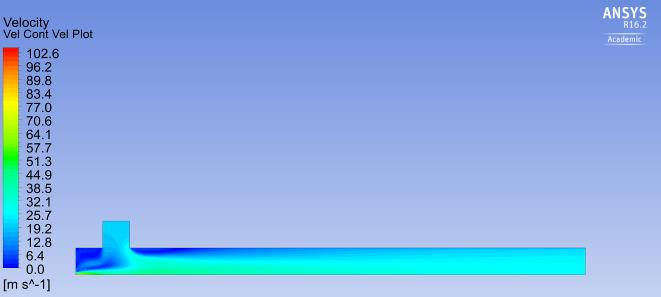
\includegraphics[width=\textwidth]{appendix/vel_ref}
        \caption{Reference velocity.}
        \label{fig:vel_ref}
\end{figure}
\begin{figure}[H]
    	\centering
        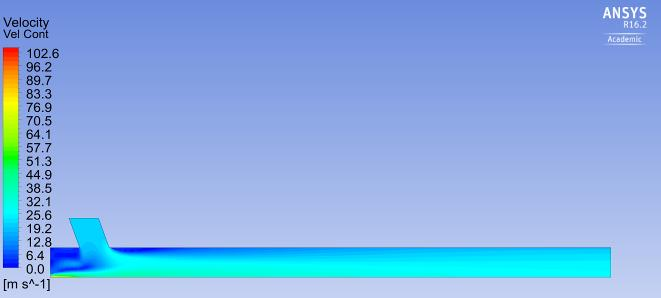
\includegraphics[width=\textwidth]{appendix/vel_mod1}
        \caption{Model 1 velocity.}
        \label{fig:vel_mod1}
\end{figure}
\begin{figure}[H]
    	\centering
        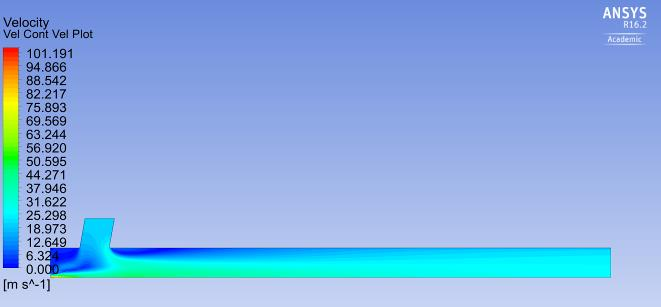
\includegraphics[width=\textwidth]{appendix/vel_mod2}
        \caption{Model 2 velocity.}
        \label{fig:vel_mod2}
\end{figure}

%------------------------------------------------------------------------------------------------------
\begin{figure}[H]
    	\centering
        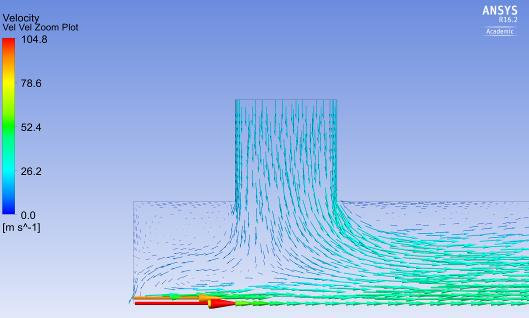
\includegraphics[width=\textwidth]{appendix/velz_ref}
        \caption{Reference velocity zoom.}
        \label{fig:velz_ref}
\end{figure}
\begin{figure}[H]
    	\centering
        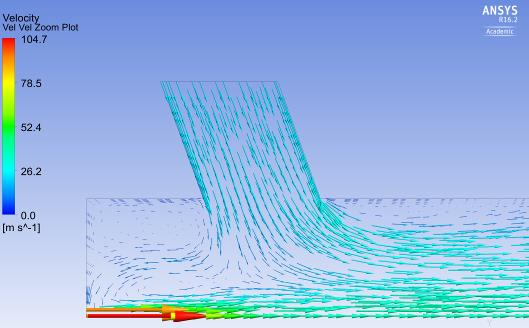
\includegraphics[width=\textwidth]{appendix/velz_mod1}
        \caption{Model 1 velocity zoom.}
        \label{fig:velz_mod1}
\end{figure}
\begin{figure}[H]
    	\centering
        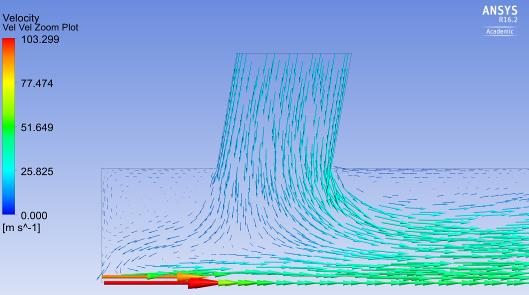
\includegraphics[width=\textwidth]{appendix/velz_mod2}
        \caption{Model 2 velocity zoom.}
        \label{fig:velz_mod2}
\end{figure}

%------------------------------------------------------------------------------------------------------
\section{Turbulent Kinetic Energy $k$}
\begin{figure}[H]
    	\centering
        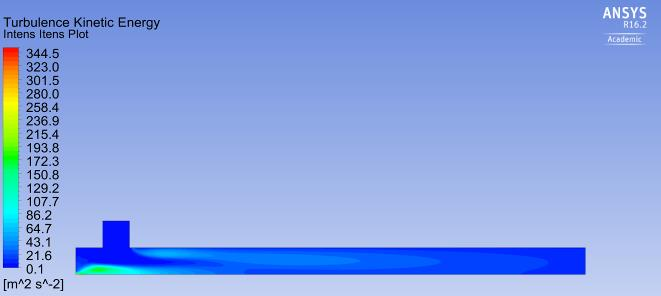
\includegraphics[width=\textwidth]{appendix/ke_ref}
        \caption{Reference turbulent kinetic energy.}
        \label{fig:ke_ref}
\end{figure}
\begin{figure}[H]
    	\centering
        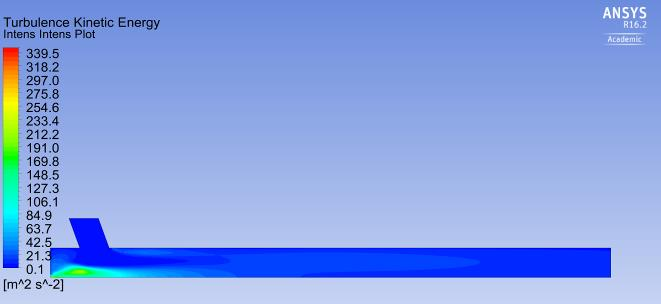
\includegraphics[width=\textwidth]{appendix/ke_mod1}
        \caption{Model 1 turbulent kinetic energy.}
        \label{fig:ke_mod1}
\end{figure}
\begin{figure}[H]
    	\centering
        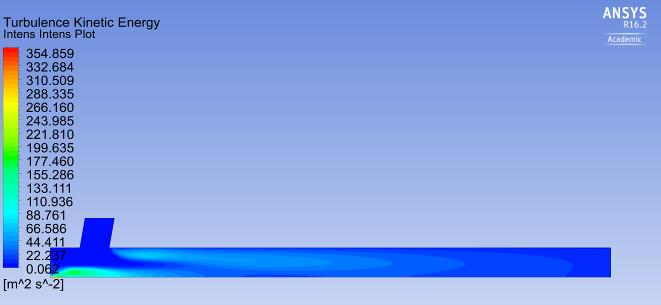
\includegraphics[width=\textwidth]{appendix/ke_mod2}
        \caption{Model 2 turbulent kinetic energy.}
        \label{fig:ke_mod2}
\end{figure}

%------------------------------------------------------------------------------------------------------
\section{Temperature $T$}
\begin{figure}[H]
    	\centering
        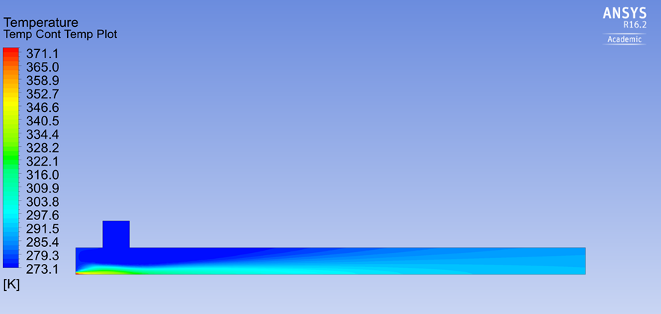
\includegraphics[width=\textwidth]{appendix/temp_ref}
        \caption{Reference temperature.}
        \label{fig:temp_ref}
\end{figure}
\begin{figure}[H]
    	\centering
        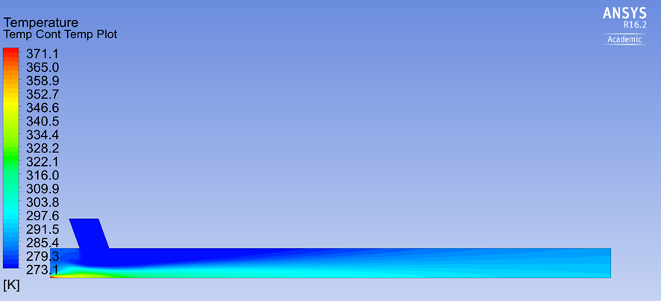
\includegraphics[width=\textwidth]{appendix/temp_mod1}
        \caption{Model 1 temperature.}
        \label{fig:temp_mod1}
\end{figure}
\begin{figure}[H]
    	\centering
        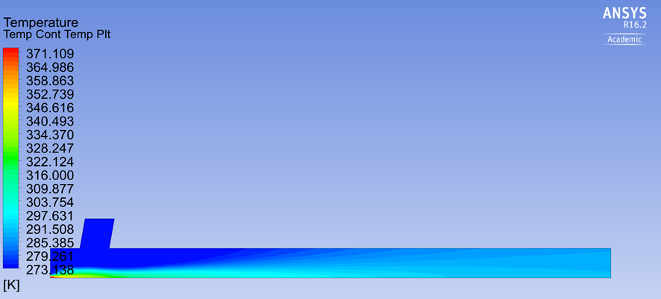
\includegraphics[width=\textwidth]{appendix/temp_mod2}
        \caption{Model 2 temperature.}
        \label{fig:temp_mod2}
\end{figure}


%------------------------------------------------------------------------------------------------------
\chapter{Appendix B: MATLAB Script}
\label{appendix:matlab}
\hypertarget{appendixb}{}
\nopagebreak
\begin{scriptsize}
	\lstinputlisting[language=MATLAB]{"C:/Users/Sebastien/Documents/GitHub/ME566/Project/MATLAB/data.m"}
\end{scriptsize}
%%%%%% --------------------------------------------------------------------------------

\end{document}
%%%%% --------------------------------------------------------------------------------
